\subsection{Programmflussdiagramm main.c}

Abbidung \ref{fig:Software_Programmflussdiagramm} zeigt den Hauptprogrammfluss vom Start des Programms über die Initialisierung des \textmu C bis in den Mainloop.

Der Aufbau der Software gliedert sich klassisch nach folgendem Prinzip. Die aufgelisteten Punkte werden in Kapitel \ref{subsec:Software_Dokumentation} beschrieben.

\begin{tabbing}

\parbox[t]{.3\textwidth}{

Modulrumpf

} \=\parbox[t]{.7\textwidth}{

Einlesen der Headerfiles.\\
Präprozessor-Anweisungen.\\
Deklarationen.\\

}\\

\parbox[t]{.3\textwidth}{Mainloop} \=\parbox[t]{.7\textwidth}{

Initialisierungen.\\
Mainroutine.

}
\end{tabbing}

\begin{figure}[h!]
	\centering	
	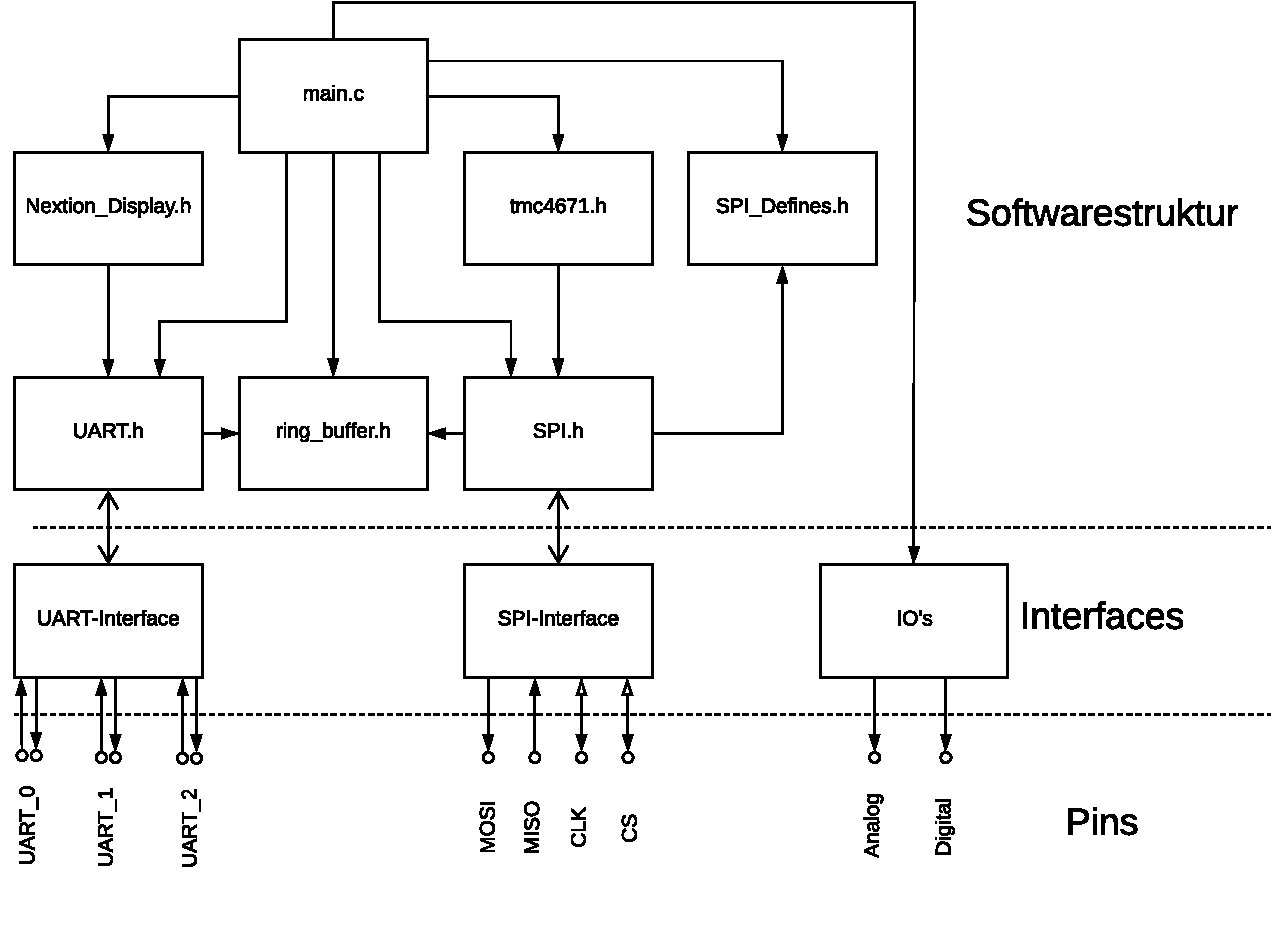
\includegraphics[width=\textwidth]{graphics/Softwarestruktur.pdf}
	\caption{Softwarestruktur Mikrocontroller.} 
	\label{fig:Software_Programmflussdiagramm}
\end{figure}

\newpage
\begin{figure}[h!]
	\centering	
	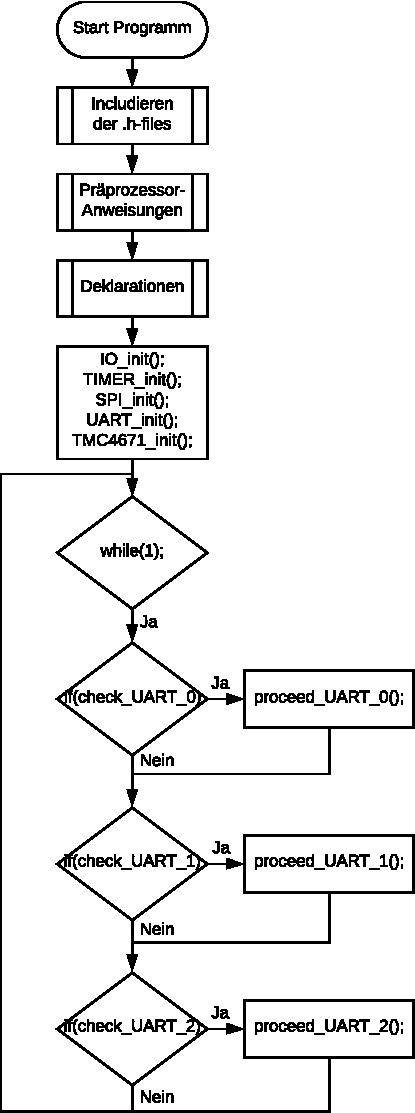
\includegraphics[width=0.52\textwidth]{graphics/Programmfluss_P5.pdf}
	\caption{Programmfluss main.c.} 
	\label{fig:Software_Programmflussdiagramm}
\end{figure}

\newpage


\subsection{Dokumentation}\label{subsec:Software_Dokumentation}

Im Foldenden werden die einzelnen Teile der Software im Detail dokumentiert. Sie gliedert sich nach den in Kapitel \ref{sec:Software_Mikrocontroller} beschriebenen Aufbau der Software.

\subsubsection{Einlesen der Headerfiles}\label{subsubsec:Einlesen_Headerfiles}

Als erstes kommen die Standardheaderfiles. Sie umfassen ein Deklarations-Set, welches für einen Basisbetrieb ausgelegt ist.

%worin Deklarationen oder auch die Bitpositionen für den Mikrocontroller, wie sie gemäss ihrem Namen im Atmel-Datenblatt definiert sind. So können anstelle einer Suche nach der Bitposition einfach die gewünschten Bitnamen verwendet werden. Sie bieten unter anderem auch typedef's für Datentypen oder Funktionen wie z.B strlen(). All diese Files sind für den Basisbetrieb ausgelegt.

\begin{tabbing}

\parbox[t]{.3\textwidth}{

\#include <avr/io.h>

} \=\parbox[t]{.75\textwidth}{

Includiert AVR-spezifische IO-Deklarationen für Registernamen etc.
% (Wichtig für Initialisierung SPI, UART etc)
\\

}\\

%\parbox[t]{.3\textwidth}{\#include <util/delay.h>} \>\parbox[t]{.75\textwidth}{Includiert alle notwendigen Deklarationen für einen möglichen Delay-Betrieb. Auch für die CPU-Frequenz ist die Bibliothek von Bedeutung, da hier das Makros F\_CPU hinterlegt ist, welches essentiell für den Betrieb jedes Mikrocontroller ist.}\\

\parbox[t]{.3\textwidth}{

\#include <avr/interrupt.h>

} \>\parbox[t]{.75\textwidth}{

Includiert Interrupt Deklarationen.\\

}\\

\parbox[t]{.3\textwidth}{

\#include <util/setbaud.h>

} \>\parbox[t]{.75\textwidth}{

Includiert das Headerfile, welches helfende Makros enthält für die Kalkulation der Baudrate. \cite{klingelbiel_c_1999}\\

}\\

\parbox[t]{.3\textwidth}{

\#include <string.h>

} \>\parbox[t]{.75\textwidth}{

Includiert die Definitionsdatei, in welcher die beiden Gruppen von Funktionen für Zeichenketten deklariert wurden. \cite{doxygen_avr-libc:_2016}
}
\end{tabbing}

Nach den Standardheaders kommen die projektbezogenen Headers. Diese wurden erstellt, um die Funktionen innerhalb der Software lesbarer zu gestalten und einen logischen Softwareaufbau zu erlangen. So können die verschiedenen Teilsysteme voneinander abgekoppelt und separat implementiert werden.

\begin{tabbing}
\parbox[t]{.3\textwidth}{

\#include "...ring\_buffer.h"

} \=\parbox[t]{.7\textwidth}{

Includiert die Ringbuffer-Header. Diese wird im SPI- und UART-Header verwedet, da sie unter Anderem ein Typedef \textit{ring\_buffer\_t} enthält.% welche für die Ringbuffer-Funktion benötigt wird.
\\

}\\

\parbox[t]{.3\textwidth}{

\#include ".../UART.h" \newline \#include ".../SPI.h"

} \>\parbox[t]{.7\textwidth}{

Includiert die Kommunikations-Headers. Eine davon ist der UART-Header, die Andere ist der SPI-Header. In beiden werden zwei Buffer initialisiert, jeweils einen für die zu sendenden Daten und einer für die zu empfangenen Daten.\\

}\\

%\parbox[t]{.3\textwidth}{
%
%\#include ".../SPI\_TMC.h"
%
%} \>\parbox[t]{.7\textwidth}{
%
%Includiert den SPI\_TMC-Header für den Motorentreiber TMC4671. Diese erlaubt eine einfache Implementierung des TMC-Kommunikationsprotokolls in die Software des Mikrocontrollers. So kann in eine darin enthaltene Funktion die Registeradresse des Treibers und der dazugehörige Wert eingegeben oder ausgelesen werden, was eine einfachere Kontrolle des Motors ermöglicht. In der Library werden die Daten so aufbereitet, dass sie in der richtigen Reihenfolge beim Treiber ankommen.\\
%
%}\\
%
\parbox[t]{.3\textwidth}{

\#include ".../TMC4671.h"

} \>\parbox[t]{.7\textwidth}{

Includiert die Befehls-Bibliothek des TMC4671. Diese enthält einige Funktionen aus der SPI\_TMC-library. Sie ermöglicht eine kompakte Befehserteilung, da je nach Ansteuerung des Motors mehrere Register des Treibers beschrieben werden müssen. Folglich ist es sinnvoll, diese in einer Funktion zu vereinen, was in diesem Header geschieht.\\

}\\

\parbox[t]{.3\textwidth}{

\#include ".../Nextion.h"

} \>\parbox[t]{.7\textwidth}{

Includiert die Befehls-Bibliothek des Nextion\_Display. Diese enthält einige Funktionen, um das Display anzusteuern. Sie ermöglicht eine bisher einigermassen kompakte Befehserteilung, da der Wrapper noch nicht fertiggestellt ist. Einige eigens geschriebene Funktionen sind jedoch schon tauglich für die Software.

}
\end{tabbing}

\subsubsection{Präprozessor-Anweisungen}\label{subsubsec:Präprozessor-Anweisungen}

Die Präprozessor-Anweisungen werden noch vor dem eigentlichen Kompilieren umgesetzt. Dabei handelt es sich um Makros (\#define) und Headerdateien (\#include).

\begin{tabbing}
\parbox[t]{.3\textwidth}{

In-/Outputs

} \=\parbox[t]{.7\textwidth}{

Hier werden die Pindefinitionen gemacht, wie sie während des Betriebs vorhanden sind. Dazu gehören die Pins für: SPI (MOSI, MISO, CLK, CS), UART (TX0, RX0, TX1, RX1), Pumpen 12x und Durchflussmessungen 12x.
%Hier werden nur \#defines verwendet. Das Bedeutet, dass ein Text-Ersatz erfolgt. Der Präprozessor ersetzt noch vor dem eigentlichen Kompilieren alle Macronamen (direkt nach dem \#define) mit dem Ersatztext dahinter.
\\

}\\
\parbox[t]{.3\textwidth}{

Pinnamen und Masken

} \=\parbox[t]{.7\textwidth}{

An dieser Stelle werden die verschiedenen Masken erstellt. Dies ermöglicht eine einfache Deklaration von ganzen Registern, wenn es darum geht, die In- und Outputs eines Systems zu definieren oder einzelne Zustände zu ändern. 
%Dies ist vorallem bei der Initialisierung von Bedeutung. So wird Beispielsweise der gesamte PORTB für SPI verwendet und deshalb als SPI\_PORT deklariert. Die darin vorkommenden Pinnamen werden durch deren  Pinfunktion gegeben. Beispielsweise wird der MOSI-Pin bennennt mit SPI\_MOSI.
\\

}\\

\parbox[t]{.3\textwidth}{

Makros

} \=\parbox[t]{.7\textwidth}{

Makros werden nur gerade zwei im Präprozessor deklariert. Diese sind dazu da, die benötigten SPI-Slaves auszuwählen. So wird in der einen Funktion der entsprechende Pin auf GND gezogen und mit der zweiten wieder auf 5V gebracht.

}

\end{tabbing}

\subsubsection{Deklarationen}\label{subsubsec:Deklarationen}

An dieser Stelle werden die für den Programmfluss nötigen Variabeln, Funktionen und Buffer vordeklariert. Dabei geht es vorallem um Variabeln zur Verarbeitung der Kommunikationsdaten.

\begin{tabbing}
\parbox[t]{.3\textwidth}{

Variabeln

} \=\parbox[t]{.7\textwidth}{

Hier werden die Variabeln deklariert, welche für den Programmfluss benötigt werden. Diese umfassen bisher Variabeln für SPI- und UART-Kommunikation sowie bufferspezifische Variabeln des Typs \textit{ring\_buffer\_t}.\\
%\begin{itemize}
%\item SPI
%\begin{itemize}
%\item volatile int cntr\_SPI = 0;
%\item volatile char INPUT\_SPI[256];
%\item volatile int SPI\_received\_finished = 0;
%\end{itemize}
%\item UART
%\begin{itemize}
%\item volatile int cntr\_UART = 0;
%\item volatile char INPUT\_UART[256];
%\item volatile int UART\_recieved\_finished = 0;
%\end{itemize}
%\end{itemize}
}\\

\parbox[t]{.3\textwidth}{

Funktionen

} \>\parbox[t]{.7\textwidth}{

In diesem Abschnitt werden Funktionen vordeklariert, welche im main.c vorkommen. Diese umfassen Funktionen für die Deklaration der IO-Ports, für die Funktion des Buffers, für das Polling ob eine komplette Datenübertragung stattgefunden hat (komplett bedeutet in diesem Fall, dass ein Ende gemäss Kommunikationsprotokoll erreicht wurde), für die Verarbeitung der Daten im Falle einer kompletten Übertragung und für ein Blinklicht, um den Status des Mikrocontrollers zu erkennen.
%\begin{itemize}
%\item Main
%\begin{itemize}
%\item IO\_Init
%\end{itemize}
%\item SPI
%\begin{itemize}
%\item void SPI\_w\_completed();
%\item extern void (*ptr\_SPI\_w\_completed)();
%\end{itemize}
%\item UART
%\begin{itemize}
%\item void tx\_completed();
%\item extern void (*ptr\_tx\_completed)();
%\end{itemize}
%\end{itemize}
}

%\parbox[t]{.3\textwidth}{
%
%Buffer
%
%} \>\parbox[t]{.7\textwidth}{
%
%Hier werden nur rein bufferspezifische Variabeln des Typs \textit{ring\_buffer\_t} deklariert.

%\begin{itemize}
%\item SPI
%\begin{itemize}
%\item ring\_buffer\_t rb\_SPI\_r;
%\item ring\_buffer\_t rb\_SPI\_w;
%\end{itemize}
%\item UART
%\begin{itemize}
%\item ring\_buffer\_t rb\_tx;
%\item ring\_buffer\_t rb\_rx;
%\end{itemize}
%\end{itemize}

%}\\

\end{tabbing}
\subsubsection{Initialisierungen}\label{subsubsec:Initialisierungen}

Im Mainloop wird, noch vor der while(1)-Schleife, als erstes die Funktion für die Initialisierung der IO-Ports aufgerufen, dann die Initialisierung der Kommunikatiosschnittstellen und zuletzt die Initialisierung des Motorentreibers. Diese werden im Folgenden erklärt:

\begin{tabbing}

\parbox[t]{.3\textwidth}{

IO-Ports

} \=\parbox[t]{.7\textwidth}{

Initialisiert die In-/Outputs, basierend auf den Definitionen im Standardheader <avr/io.h> und in den Präprozessor-Anweisungen. Die Initialisierung an sich wird in der Funktion void IO\_Init(void) aufgerufen.\\

}\\

\parbox[t]{.3\textwidth}{

SPI

} \=\parbox[t]{.7\textwidth}{

Initialisiert die SPI-Schnittstelle. Massgebend ist das SPI Control Register (SPCR). Dieses wurde nach SPI-Mode 3, MSB first und 1MHz konfiguriert und entspricht so den Anforderungen des Motorentreibers, welcher über SPI angesteuert wird. Die Funktion zur Initialisierung der SPI-Schnittstelle heisst SPI\_init().\\

}\\

\parbox[t]{.3\textwidth}{

UART

} \=\parbox[t]{.7\textwidth}{

Initialisiert die UART-Schnittstelle. Massgebend sind die Register UCSRnB und UCSRnC bzw. UCSRnB und UCSRnC. Die Variable n im Registername steht für den UART-Port n, da der Atmega2560 mehrere UART-Schnittstellen hat. Da drei UART-Ports benötigt werden, wird die Reihenfolge der Schnittstellen foldendermassen festgelegt: UART-Port 0 = USB, UART-Port 1 = Nextion-Display. Für eine Ertweiterung mit einem WLAN-Modul wird UART- Port 2 verwendet.

Die Register UBRRnH und UBRRnL definieren die Baudrate der Kommunikation. Mit der Bibliothek <util/setbaud.h> kann der Wert mit UBRRH\_VALUE und UBRRL\_VALUE angegeben werden. Die beiden Werte werden mit einem Makros berechnet.\\

}\\

\parbox[t]{.3\textwidth}{

TMC4671

} \=\parbox[t]{.7\textwidth}{

Initialisiert den TMC4671. Im Gegensatz zu den vorherigen Initialisierungen  geht es bei dieser Initialisierung nicht darum, etwas im Mikrocontroller zu initialisieren, sondern der Motorentreiber wird auf die Treiberschaltung des AKM22h und den AKM22h an sich initialisiert. Dazu werden die entsprechenden Register beschrieben, welche durch Verwendung der Trinamic-Software \textit{TMCL-IDE 3.0} ermittelt wurden.\\

}\\

\parbox[t]{.3\textwidth}{

Ring Buffer

} \=\parbox[t]{.7\textwidth}{

%Da bei allen Schnittstellen sende- und empfangsseitig mit einem Ring-Buffer gearbeitet wird, werden diese Buffer auch im UART\_init() initialisiert. Dazu wird die Ring\_Buffer.h-Library verwendet, worin auch die Funktion \textbf{RB\_init(ring\_buffer\_t);} existiert. Weiteres zu dieser Funktion wird im Kapitel \ref{Appendix:TMC4671}\todo{Referenzierung ändern, auf Ring\_Buffer referenzieren.}

Für jede Schnittstelle wird sende- und empfangsseitig mit einem Ring Buffer gearbeitet. Diese müssen auch jeweils initialisiert werden, was mittels einer Funktion der Bibliothek Ring\_Buffer.h geschieht. Die gemeinte Funktion heisst RB\_init(ring\_buffer\_t);. Der Buffer verhindert einen Datenstau aufgrund zu langsamer Datenverarbeitung im Mikrocontroller. Die Daten werden im Buffer zwischengespeichert und können verarbeitet werden, sobald der Mikrocontroller dazu kommt.\\

}\\

\parbox[t]{.3\textwidth}{

Interrupts

} \=\parbox[t]{.7\textwidth}{

Soweit möglich wurde bei jeder Schnittstelle mit Interrupts gearbeitet. In Kombination mit dem Buffer wird der Hauptprogrammfluss nur wenig gestört und erlaubt trotzdem eine zuverlässige Verarbeitung der einkommenden Daten. Die globalen Interrupts müssen jeweils mit sei(); aktiviert werden.

}

\end{tabbing}

%\begin{itemize}
%\item Enable SPI-Interface
%\begin{itemize}
%\item (1<<SPE)
%\end{itemize}
%\item Enable SPI-Interrupt
%\begin{itemize}
%\item (1<<SPIE)
%\end{itemize}
%\item Act as Master
%\begin{itemize}
%\item (1<<MSTR)
%\end{itemize}
%\item SPI Mode 3
%\begin{itemize}
%\item (1<<CPOL)|(1<<CPHA)
%\end{itemize}
%\item Clock 1MHz
%\begin{itemize}
%\item (1<<SPR1)|(1<<SPR0)
%\end{itemize}
%\item MSB first
%\begin{itemize} 
%\item (0<<DORD)
%\end{itemize}
%\end{itemize}

%\begin{equation}
%UBRR = \frac{Taktfrequenz (in Hz)}{16 \cdot Baudrate} - 0.5
%\end{equation}

%Dieser Wert wird dann auf ein Higher und ein Lower-Byte aufgeteilt, welche wiederum die Register UBRRH\_VALUE und UBRRL\_VALUE definieren. 

%UCSR0B/UCSR1B:
%\begin{itemize}
%\item TX-/RX aktivieren
%\begin{itemize}
%\item (1<<RXEN0)
%\item (1<<TXEN0)
%\item (1<<RXEN1)
%\item (1<<TXEN1)
%\end{itemize}
%\item UART RX-Interrupt setzen
%\begin{itemize}
%\item (1<<RXCIE0)
%\item (1<<RXCIE1)
%\end{itemize}
%\end{itemize}
%
%UCSR0C/UCSR1C
%\begin{itemize}
%\item 8 Bits pro Übertragungsmenge
%\begin{itemize}
%\item (1<<UCSZ00)
%\item (1<<UCSZ01)
%\item (1<<UCSZ10)
%\item (1<<UCSZ11)
%\end{itemize}
%\end{itemize}



%Da während des Betriebs die Sende- und Empfangskanäle dekativiert werden sollen, wurden zwei Präprozessor-Funktionen definiert, welche genau dieses Ein- und Ausschalten ausführt. Die einschaltende Funktion \textbf{Uart\_EnableRxIT();} wurde als Sicherheit in die Initialisierung mitgeschrieben, damit der Datenempfang gewährleistet ist.

%Um die Initialisierung zu testen, wird ein Test-Text per UART0 (USB-Schnittstelle) eine Zeichenkette ausgesendet. Dazu wird der Pointer auf den String vorsorglich auf Null gesetzt und dann die Daten mittels Uart\_Transmit\_IT("TestText",länge String); an den Empfänger gesendet.

\subsubsection{Mainroutine}\label{subsubsec:Mainroutine}

In der Mainroutine wird bisher nur geprüft, ob die Buffer Daten enthalten. Sobald bei einkommenden Daten das Ende einer Übertragung signalisiert erkannt wird, werden diese in einer weiteren Funktion ausgewertet.

%Die Buffer werden ausgelesen, sobald deren enthaltene Datenmenge grösser als Null ist. Die Ablaufprogramme werden aufgerufen, nachdem der Inhalt der empfangenen Daten ausgelesen und interpretiert wurden.

\subsection{libraries}\label{subsec:Software_Lib}

Damit das lauffähige Programm eine Struktur aufweist und der Code übersichtlich bleibt, werden die verschiedenen Aufgabebereiche in Libraries geschrieben. Diese werden zu Beginn des Programmes eingefügt, um die darin enthaltenen Funktionen verwenden zu können.

Zu den Libraries gehören die SPI-, SPI-TMC, UART-, Ring\_Buffer- und die TMC4671- Library. Diese fünf libraries werden im Folgenden kurz erklärt.

\subsubsection{Ring Buffer}\label{subsubsec:Software_RingBuffer}

In der Ring-Buffer Library befinden sich Funktionen, mit denen der Ring Buffer beschrieben und ausgelesen werden kann. Ausserdem können verschiedene Informationen zum Datenbestand innerhalb des Buffers abgefragt werden.

\begin{enumerate}
\item void RB\_init(ring\_buffer\_t *rb);
\item unsigned char	RB\_free(ring\_buffer\_t *rb);
\item unsigned char	RB\_length(ring\_buffer\_t *rb);
\item unsigned char	RB\_readByte(ring\_buffer\_t *rb);
\item unsigned char	RB\_writeByte(ring\_buffer\_t *rb, unsigned char data);
\item unsigned char	RB\_read(ring\_buffer\_t *rb, unsigned char *data, unsigned char datal);
\item unsigned char	RB\_write(ring\_buffer\_t *rb, unsigned char *data, unsigned char datal);
\end{enumerate}

Die Funktionen haben folgende Aufgaben bzw. führen folgende Aufgaben aus:

\begin{enumerate}
\item Initialisiert einen neuen Buffer.
\item Gibt die Anzahl freier Plätze im Buffer zurück.
\item Gibt die Anzahl belegter Plätze im Buffer zurück.
\item Liest und löscht ein Byte aus dem Buffer.
\item Schreibt ein Byte in den Buffer.
\item Liest mehrere Bytes aus dem Buffer aus.
\item Schreibt mehrere Bytes in den Buffer rein.
\end{enumerate}

\subsubsection{SPI}\label{subsubsec:Software_SPI}

Wie beschrieben wird die SPI-Library verwendet, um Daten über das Serial Peripheral Interface zu versenden. Dazu wird die SPI-Library verwendet, welche folgende Funktionen beinhaltet:

\begin{enumerate}
\item void SPI\_init(void);
\item SPI\_Transmit\_IT(unsigned char * data, unsigned char nbytes);
\item ISR(SPI\_STC\_vect);
\end{enumerate}

Die Funktionen haben folgende Aufgaben bzw. führen folgende Aufgaben aus:

\begin{enumerate}
\item Initialisiert die Hardware sowie Ring-Buffer für die Empfangs- siwue Sendeseite.
\item Füllt den Buffer mit zu übertragenden Daten und schreibt die Daten aus dem Buffer wieder in das Datenregister der SPI-Schnittstelle. Dies geschieht für ein Byte, die noch im Buffer vorhandenen Bytes werden für die Übertragung über die Interrupt-Routine gehandelt, welche ausgelöst wird sobald das erste Byte an den Slave gesendet wurde.
\item Interrupt-Routine: Falls Daten im Schreib-Buffer des SPI sind, sollen diese Byte-weise in das SPI-Datenregister geschrieben werden. Sind keine Daten vorhanden, soll nichts gemacht werden.
\end{enumerate}

\subsubsection{UART}\label{subsubsec:Software_UART}

Auch die UART-Library wurde schon erklärt. So ist die Schnittstelle dafür da, Daten über die Universelle Asynchrone Receiver-/Transmitter schnittstelle zu senden. Es ist eine gängige Schnittstelle, welche über ein USB-Kabel realisiert werden kann. Sie ermöglicht also eine Verbindung zu einem Computer.

Die Library an sich beinhaltet folgende Funktionen:

\begin{enumerate}
\item UART\_init(void);
\item UART\_Transmit\_IT\_n();
\item ISR(USARTn\_UDRE\_vect);
\item ISR(USARTn\_RX\_vect);
\end{enumerate}

Die Funktionen haben folgende Aufgaben bzw. führen folgende Aufgaben aus:

\begin{enumerate}
\item Initialisiert die UART-Schnittstellen.
\item Übermittelt Daten über die gewählte UART-Schnittstelle n.
\item Sobald das UART-Interface bereit ist, neue Daten zu senden, wird dieses Interrupt ausgelöst. Solange sich Daten im Sende-Buffer befinden, werden diese nach und nach über die UART-Schnittstelle versendet.
\item Sobald Daten über die UART-Schnittstelle empfangen wurden, wird diese Interruptroutine ausgelöst. Darin werden die empfangenen Daten in den Buffer zwischengespeichert.
\end{enumerate}

\subsubsection{TMC4671}\label{subsubsec:Software_TMC4671}

In der Library für den TMC4671 sind Funktionen enthalten, mit denen der Treiber über SPI initialisiert und angesteuert werden kann. Die wichtigsten Funktionen darin sind diejenigen, welche gewährleisten, dass der Treiber die Daten in der richtigen Reihenfolge empfängt. Sie sind im Folgenden aufgelistet. So kann einer Funktion eine Adresse mit zugehörigem Wert mitgegeben werden. Innerhalb der Funktion werden die Daten der richtige Reihenfolge nach in einem Array abgelegt und über die Sendefunktion der SPI-Library über die gleichnamige Schnittstelle versendet. 

Es befinden sich nebst diesen Sendefunktionen noch mehr Funktionen darin, mit denen die Parameter des TMC4671 eingestellt werden können. Die Funktionen enthalten in der Regel die gewünschte Adresse des Zielparameters und eine der Sendefunktionen, womit der Zielparameter übermittelt und in den Treiber geladen wird. Von diesen Funktionen sind auch einige aufgelistet, welche für die Cocktailmaschine von Bedeutung sein können.

Um zu verstehen, wie die wichtigen Funktionen aufgebaut sind, muss geklärt werden, nach welcher Datenfolge der Motorentreiber arbeitet. Im Datenblatt vom Trinamic TMC4671 wurden folgende Informationen gefunden:

\begin{itemize}
\item 40-bit Datagrammlänge (1 ReadWrite-Bit, 7 Adress-Bits + 32 Daten-Bits).
\item Sofortige SPI-Leseantwort (Registerlesezugriff über ein einziges Datagramm).
\item SPI-Clock-Frequenz bis 1MHz (8MHz in zukünftigen Versionen).
\end{itemize}

\begin{figure}[h!]
	\centering
	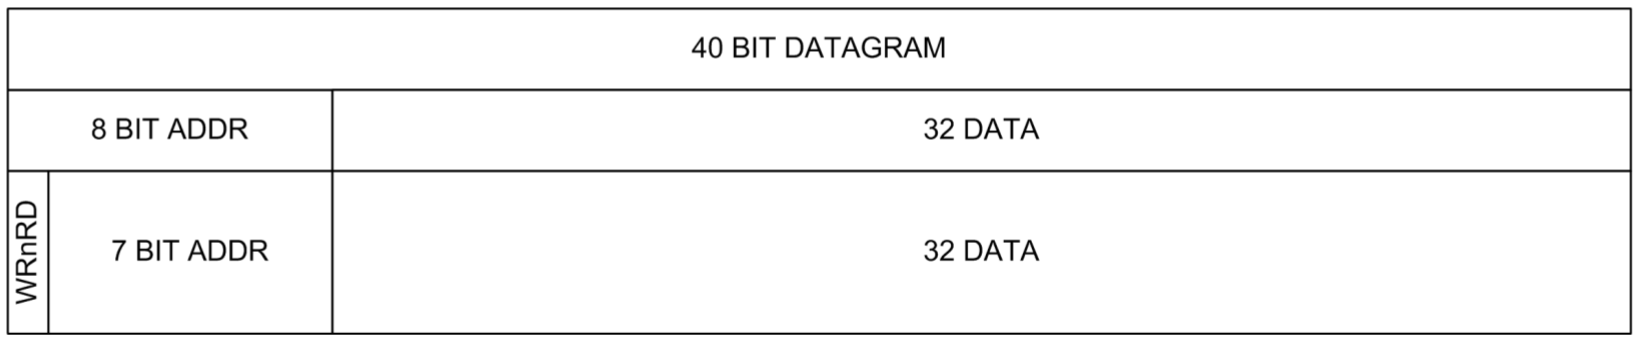
\includegraphics[width=0.8\textwidth]{graphics/SPI_Datagramm.png}
	\caption{SPI-Datenstruktur.
	\cite{trinamic_datasheet_2018}}
	\label{fig:SPI_Datenstruktur}
\end{figure}

In den aufgelisteten Funktionen befindet sich jeweils der Parameter ``unsigned int motor``. Dessen Funktion ist unbekannt, es wird jedoch vermutet, dass diese Einstellung für einen Treiber bestimmt ist, welcher mehrere Motoren ansteuern kann. Um die Funktionalität der Funktionen zu gewährleisten, wurde dieser Parameter jeweils mit ``\#define MOTOR0 0`` deklariert und geladen. Die wichtigen Funktionen sind im folgenden aufgelistet und können als ``SPI-Wrapper`` betrachtet werden, welcher die Verbindung zwischen der SPI-Library und der TMC4671-Library bildet: \cite{noauthor_tmc-evalsystem/tmc4671_eval.c_nodate}

\begin{enumerate}
%\item void tmc4671\_writeDatagram(unsigned int motor, unsigned char address, unsigned int x1, unsigned int x2, unsigned int x3, unsigned int x4);
%\item void tmc4671\_writeInt(unsigned int motor, unsigned char address, unsigned long value);
%\item int tmc4671\_readInt(unsigned int motor, unsigned char address);
\item void tmc40bit\_writeInt(unsigned int motor, unsigned char address, unsigned long value);
\item int tmc40bit\_readInt(unsigned int motor, unsigned char address);
\end{enumerate}

%Bei der Beschreibung ist zu erkennen, dass die Library für das Lesen und Schreiben zwei Funktionen beihnaltet, welche die selbe Funktion haben. Die Funktionen (2.) und (3.) beinhalten sogar nur die Funktionen (4.) und (5.). Der eigentrliche ``Wrapper`` besteht folglich rein aus den Funktionen (4.) und (5.).

%Für eine Implementierung eines anderen Treibers oder Motors müsste man hier weiterarbeiten, was jedoch nicht Teil dieses Projektes ist.

Im Falle der Cocktailmaschine docken wir uns hier mit der Funktion ``tmc40bit\_(read/write)Int`` der TMC4671-Library und der Fonktion ``SPI\_Transmit\_IT`` an die SPI-Library des Miktrocontrollers. Nun können die restlichen Funktionen der TMC4671-Library verwendet werden, ohne im Programmfluss die SPI-Library verwenden zu müssen. Ausnahme: Chip-Select des Treibers auf enable/disable setzen.

\begin{enumerate}
%\item Schreibt ein Datagramm mit fünf selbst definierten Bytes.
%\item Schreibt eine 8-Bit Adresse mit einem folgenden 24-Bit Wert.
%\item Schreibt eine 8-Bit Adresse und liest einen 24-Bit Wert zurück.
\item Schreibt eine 8-Bit Adresse mit einem folgenden 24-Bit Wert.
\item Schreibt eine 8-Bit Adresse und liest einen 24-Bit Wert zurück.
\end{enumerate}

\subsubsection{Nextion Display}\label{subsubsection:Software_Nextion}

Die offizielle Library für das Nextion-Display wurde nicht verwendet, da sie in C++ geschrieben ist. Auch eine veröffentlichte Version auf GitHub, welche in C geschrieben worden war, stellte sich als zu kompliziert heraus. Deswegen wurde bisher versucht, eine vereinfachte Library zu schreiben. Sie basiert auf dem gleichen Prinzip wie die SPI-Library: Es wird ein Wrapper geschrieben, welcher sich nach dem Kommunikationsprinzip des Displays richtet. Bei Bedarf kann so eine Funktion geschrieben werden, welche einen Datenaustausch zwischen Mikrocontroller und Display auslöst. Leider ist dies beim Nextion-Display aufwendiger aufgrund unterschiedlich langen Übertragunsarrays. Deshalb wird diese eine Aufgabe für das Projekt sechs sein.

\subsection{Lizenzen Bibliotheken}\label{subsec:Software_Lizenzen}


\subsubsection{SPI}\label{subsubsec:Software_Lizenzen_SPI}

Die SPI-Library wurde selbst geschrieben. Lediglich die Methodik mit dem RingBuffer wurde aus der UART-Library auf das SPI angewendet. Somit könnte man sagen, dass die Idee von dort stammt.
\cite{user_ring_nodate}

\subsubsection{Uart}\label{subsubsec:Software_Lizenzen_UART}

Die UART-library enthält keine spezifisch definierte Lizenz. Die Bibliothek wurde zusammen mit der RingBuffer-Librarygefunden auf Youtube. In der Videobeschreibung gibt es einen Link, mit dem man die Bibliothek runterladen kann. Der Autor heiss Jr Sf.
\cite{user_ring_nodate}

\subsubsection{Ring-Buffer}\label{subsubsec:Software_Lizenzen_Ring_Buffer}

Die RingBuffer-library enthält keine spezifisch definierte Lizenz. Die Bibliothek wurde zusammen mit der UART-Library gefunden auf Youtube. In der Videobeschreibung gibt es einen Link, mit dem man die Bibliothek runterladen kann. Der Autor heiss Jr Sf.
\cite{user_ring_nodate}

\subsubsection{TMC4671}\label{subsubsec:Software_Lizenzen_TMC4671}

Die Library stammt von Trinamic. Folgende Lizenz wurde erwähnt:

MIT License

Copyright (c) 2019 Trinamic Motion Control GmbH \& Co. KG

Permission is hereby granted, free of charge, to any person obtaining a copy
of this software and associated documentation files (the "Software"), to deal
in the Software without restriction, including without limitation the rights
to use, copy, modify, merge, publish, distribute, sublicense, and/or sell
copies of the Software, and to permit persons to whom the Software is
furnished to do so, subject to the following conditions:

The above copyright notice and this permission notice shall be included in all
copies or substantial portions of the Software.

THE SOFTWARE IS PROVIDED "AS IS", WITHOUT WARRANTY OF ANY KIND, EXPRESS OR
IMPLIED, INCLUDING BUT NOT LIMITED TO THE WARRANTIES OF MERCHANTABILITY,
FITNESS FOR A PARTICULAR PURPOSE AND NONINFRINGEMENT. IN NO EVENT SHALL THE
AUTHORS OR COPYRIGHT HOLDERS BE LIABLE FOR ANY CLAIM, DAMAGES OR OTHER
LIABILITY, WHETHER IN AN ACTION OF CONTRACT, TORT OR OTHERWISE, ARISING FROM,
OUT OF OR IN CONNECTION WITH THE SOFTWARE OR THE USE OR OTHER DEALINGS IN THE
SOFTWARE.

\cite{noauthor_trinamictmc-evalsystem_nodate}